% Prophet's MAP estimate is not the posterior mode.
% Preprint, intended for arXiv stat.CO.  Build with `make` in this directory.
\documentclass[11pt]{article}

\usepackage[margin=1in]{geometry}
\usepackage[T1]{fontenc}
\usepackage{lmodern}
\usepackage{microtype}
\usepackage{amsmath,amssymb,amsthm}
\usepackage{graphicx}
\usepackage{booktabs}
\usepackage{xcolor}
\usepackage[round,sort&compress]{natbib}
\usepackage[colorlinks=true,linkcolor=blue!50!black,citecolor=blue!50!black,
            urlcolor=blue!50!black]{hyperref}
\usepackage[capitalise,noabbrev]{cleveref}

% Identifiers and paths, breakable at / _ . and - so a long name never overruns
% the margin. hyperref loads `url`, which provides \path.
\def\UrlBreaks{\do\/\do\_\do\.\do\-}
\newcommand{\code}[1]{\path{#1}}

% Every number the prose quotes is generated from the committed results by
% experiments/quote_numbers.py. None is typed here by hand.
% Generated by paper/experiments/quote_numbers.py from the committed
% evaluation results. Do not edit: rerun the script.

\newcommand{\CensusDaily}{2,714}
\newcommand{\CensusDigest}{ab399af9181e}
\newcommand{\CensusSeries}{3,008}
\newcommand{\CensusWeekly}{294}
\newcommand{\KktKinkRate}{6.5\times10^{-8}}
\newcommand{\KktLpMedian}{5.0}
\newcommand{\KktLpMin}{0.06}
\newcommand{\KktLpWins}{3,008}
\newcommand{\KktOursMedian}{0.17}
\newcommand{\KktOursWorst}{2.5}
\newcommand{\KktPeytonOurs}{0.10}
\newcommand{\KktPeytonProphetRelaxed}{4.1}
\newcommand{\KktPeytonProphetStrict}{26.7}
\newcommand{\KktProphetRelaxed}{9.8}
\newcommand{\KktProphetRelaxedMin}{1.3}
\newcommand{\KktProphetStrict}{52}
\newcommand{\KktRatio}{59}
\newcommand{\KktRatioMin}{4.0}
\newcommand{\KktRelaxedAtRate}{66}
\newcommand{\KktRelaxedAtTrend}{31}
\newcommand{\KktSeries}{3,008}
\newcommand{\KktStrictAtRate}{99}
\newcommand{\KktWorse}{3,008}
\newcommand{\LimBestCensus}{54.6}
\newcommand{\LimCoverageOurs}{0.345}
\newcommand{\LimCoverageProphet}{0.341}
\newcommand{\LimDailyModalShare}{55}
\newcommand{\LimDailyStarts}{122}
\newcommand{\LimHolmComparisons}{six}
\newcommand{\LimHolmMax}{3.7\times10^{-19}}
\newcommand{\LimHolmMin}{3.1\times10^{-105}}
\newcommand{\LimHolmSurvivors}{six}
\newcommand{\LimMfourFrequencies}{six}
\newcommand{\LimMfourSeries}{100,000}
\newcommand{\LimNewtonLength}{50}
\newcommand{\LimNewtonShare}{9}
\newcommand{\LimNewtonSpeedup}{7.5}
\newcommand{\LimOverheadShareMax}{54}
\newcommand{\LimOverheadShareMin}{24}
\newcommand{\LimParityMax}{1.1}
\newcommand{\LimParityMin}{0.9}
\newcommand{\LimPoolSize}{658}
\newcommand{\LimPoolThreshold}{0.10}
\newcommand{\LimWeeklyFutureStarts}{43}
\newcommand{\LimWidthMedian}{2.47}
\newcommand{\LimWidthWider}{2,153}
\newcommand{\LimWorstCensus}{325}
\newcommand{\LimWorstPool}{78.7}
\newcommand{\LpDecline}{54}
\newcommand{\LpMarginLong}{+0.361}
\newcommand{\LpMarginMid}{+2.760}
\newcommand{\LpMarginShort}{+1.986}
\newcommand{\LpPercentLong}{0.0045}
\newcommand{\LpPercentMid}{0.0968}
\newcommand{\LpPercentShort}{0.2442}
\newcommand{\MarginAfterYearly}{0.12}
\newcommand{\MarginAtHundred}{0.72}
\newcommand{\MarginAtNinetyNine}{0.018}
\newcommand{\MarginBeforeYearly}{0.93}
\newcommand{\MarginCells}{126}
\newcommand{\MarginLbfgsMax}{4.3}
\newcommand{\MarginLbfgsMedian}{1.2}
\newcommand{\MarginLbfgsMin}{0.11}
\newcommand{\MarginLengths}{79}
\newcommand{\MarginNewtonMedian}{0.0088}
\newcommand{\MarginYearlyFrom}{693}
\newcommand{\MarginYearlyLong}{+2.34}
\newcommand{\NewtonFlipsMax}{9,549}
\newcommand{\NewtonFlipsMin}{1,022}
\newcommand{\NewtonIterMax}{1,409}
\newcommand{\NewtonIterMin}{240}
\newcommand{\NewtonLengthMax}{2905}
\newcommand{\NewtonLengthMin}{50}
\newcommand{\NewtonLengths}{six}
\newcommand{\NewtonProgressMax}{9.8\times10^{-6}}
\newcommand{\NewtonProgressMin}{2.6\times10^{-6}}
\newcommand{\NewtonShortMax}{7.1}
\newcommand{\NewtonShortMin}{1.2}
\newcommand{\NewtonSplitIterMax}{528}
\newcommand{\NewtonSplitIterMin}{44}
\newcommand{\NewtonSplitZerosMax}{25}
\newcommand{\NewtonSplitZerosMin}{15}
\newcommand{\NewtonStanMax}{0.21}
\newcommand{\NewtonStanMin}{0.0021}
\newcommand{\RmseAdvantage}{0.40}
\newcommand{\RmseWinRate}{64}
\newcommand{\RmseWins}{1,929}
\newcommand{\SmoothBestEpsLong}{10^{-4}}
\newcommand{\SmoothBestEpsMid}{10^{-5}}
\newcommand{\SmoothBestEpsShort}{10^{-5}}
\newcommand{\SmoothBestLong}{0.046}
\newcommand{\SmoothBestMid}{0.0029}
\newcommand{\SmoothBestShort}{0.0012}
\newcommand{\SmoothCrossingLong}{1.4\times10^{-3}}
\newcommand{\SmoothCrossingMid}{2.9\times10^{-5}}
\newcommand{\SmoothCrossingShort}{7.1\times10^{-6}}
\newcommand{\SmoothDecrementMax}{3.0\times10^{-13}}
\newcommand{\SmoothDropLong}{15}
\newcommand{\SmoothDropMid}{1,500}
\newcommand{\SmoothDropShort}{25,000}
\newcommand{\SmoothEpsMin}{10^{-8}}
\newcommand{\SmoothFactorLong}{8}
\newcommand{\SmoothFactorMid}{941}
\newcommand{\SmoothFactorShort}{1,592}
\newcommand{\SmoothGapAtMinLong}{0.36}
\newcommand{\SmoothGapAtMinMid}{1.88}
\newcommand{\SmoothGapAtMinShort}{2.00}
\newcommand{\SmoothIterMax}{4,044}
\newcommand{\SmoothIterMin}{238}
\newcommand{\SmoothPlateauMaxLong}{0.15}
\newcommand{\SmoothPlateauMaxMid}{0.0075}
\newcommand{\SmoothPlateauMaxShort}{0.0011}
\newcommand{\SmoothPlateauMinLong}{0.025}
\newcommand{\SmoothPlateauMinMid}{0.0013}
\newcommand{\SmoothPlateauMinShort}{8.1\times10^{-5}}
\newcommand{\SmoothRuns}{51}
\newcommand{\SmoothStoppedGradient}{50}
\newcommand{\SmoothValues}{17}
\newcommand{\StallBestReach}{37}
\newcommand{\StallCondition}{142}
\newcommand{\StallLbfgsCosine}{0.996}
\newcommand{\StallLbfgsIter}{28}
\newcommand{\StallLbfgsRelaxed}{0.65}
\newcommand{\StallLbfgsShort}{0.079}
\newcommand{\StallNewtonIter}{24}
\newcommand{\StallNewtonShort}{2.0\times10^{-8}}
\newcommand{\StallOptima}{two}
\newcommand{\StallOursEigen}{-4.74}
\newcommand{\StallOursShort}{3.22}
\newcommand{\StallSecondsMax}{0.04}
\newcommand{\StallSmoothEps}{10^{-4}}
\newcommand{\StallSmoothIdentical}{0.079}
\newcommand{\StallSmoothShort}{1.0\times10^{-4}}
\newcommand{\StallStarts}{40}
\newcommand{\StallVariantIterMax}{54}
\newcommand{\StallVariantIterMin}{9}
\newcommand{\StallVariantNewtonMax}{8.1\times10^{-4}}
\newcommand{\StallVariantShortMax}{1.34}
\newcommand{\StallVariantShortMin}{0.079}
\newcommand{\StallVariants}{nine}


% The commit this PDF is built from, which `make` writes at every build. It is
% not committed, so a build that bypasses make says so rather than failing.
\InputIfFileExists{generated/build.tex}{}{\newcommand{\BuildCommit}{unrecorded}}

% A result the paper states but has not yet measured.  It renders visibly so
% that nothing unmeasured can reach a submitted version unnoticed; the build
% refuses to produce a submission while any remain (see Makefile).
\newcommand{\pending}[2]{\textcolor{red!70!black}{[\textbf{pending \projectissue{#1}}: #2]}}

% Issues are cited as links to their threads, never as bare numbers, and the
% text names the tracker as GitHub's cross-repository references do: prophet#842
% is an upstream report, analytic-prophet#193 this implementation's own issue.
% A bare #842 would leave a reader unable to tell the two apart.
\newcommand{\prophetissue}[1]{\href{https://github.com/facebook/prophet/issues/#1}{prophet\##1}}
\newcommand{\projectissue}[1]{\href{https://github.com/adlyZaroui/analytic-prophet/issues/#1}{analytic-prophet\##1}}

\theoremstyle{plain}
\newtheorem{proposition}{Proposition}
\theoremstyle{remark}
\newtheorem{remark}{Remark}

\newcommand{\T}{\ensuremath{T}}
\newcommand{\lp}{\ensuremath{\mathrm{lp}}}

\title{Prophet's MAP Estimate Is Not the Posterior Mode:\\
       A Non-Differentiable Changepoint Prior, Smooth Optimizers,\\
       and an Exact Reformulation}
\author{Adly Zaroui\\[2pt]
  {\small Independent researcher}\\[1pt]
  {\small\href{mailto:mohamed-adly.zaroui@outlook.com}%
                {\texttt{mohamed-adly.zaroui@outlook.com}}}}
\date{\today\\[2pt]{\small Built from commit \texttt{\BuildCommit}}}

\begin{document}
\maketitle

\begin{abstract}
Prophet is a widely deployed forecasting library that fits its model by maximum
a~posteriori estimation. The posterior it specifies places a Laplace prior on
the trend's changepoint rates, which makes the objective non-differentiable
exactly where its optimum tends to lie, at rates of zero. Prophet delegates the
optimization to Stan's L-BFGS and Newton methods, which are methods for smooth
objectives. We show that, as a consequence, the MAP estimate Prophet returns is not
the posterior mode: under Prophet's own posterior density it scores below the
optimum at every series length measured, and its changepoint rates never reach the
exact zeros the optimum has. On every one of \KktSeries{} M4 series,
Prophet's solution fails the first-order optimality conditions, even when each
changepoint rate is read in the way most favourable to it.
Run from \MultiTotal{} random starts on Prophet's program with $\sigma$ held fixed,
where the optimum is unique, Stan's L-BFGS with Prophet's settings reaches it from
none. The defect is diagnosable and is removed by an exact reformulation that splits
each rate into non-negative parts. Of four long-standing reports in Prophet's issue
tracker, it accounts for part of one and plausibly underlies a second; it explains
neither of the others. On a frozen census of \CensusSeries{}
held-out M4 series, the corrected optimum forecasts better on \RmseWinRate\% of
them, by a median of \RmseAdvantage\% in RMSE: the optimization defect is real,
and its cost to forecast accuracy is usually small.
\end{abstract}

\section{Introduction}
\label{sec:introduction}

Prophet \citep{taylor2018forecasting} fits a decomposable time-series model by
maximum a~posteriori (MAP) estimation. Its authors specified the model as a Stan
program \citep{carpenter2017stan} and delegated the optimization to Stan, which
runs L-BFGS by default and Newton's method on short series. The posterior they
specified places a Laplace prior on the rates by which the trend changes slope,
and a Laplace prior contributes a term $\sum_j |\delta_j|/\tau$ to the negative log
posterior. That term is not differentiable where any $\delta_j = 0$ --- and the
optimum sits there, because sending most rates to zero is precisely what the
prior is for.

Stan's reference manual describes its optimizers by pointing to
\citet{nocedal2006numerical} for ``thorough description and analysis''
\citep{stan2025reference}, a text that ``focuses on smooth functions, by which we
generally mean functions whose second derivatives exist and are continuous'' and
leaves nonsmooth optimization out of its scope. Stan's function reference does warn
that the absolute value, among other step-like functions, ``can seriously hinder
sampling and optimization efficiency for gradient-based methods (e.g., NUTS, HMC,
BFGS) if applied to parameters'' \citep{stan2025functions}. The double-exponential
distribution, whose log density contains the same absolute value, carries no such
warning, and it is through the distribution that Prophet's model reaches it.
Nothing about this arrangement is an error.
The model is reasonable, the optimizers are correctly implemented and correctly
documented, and the delegation is the ordinary way a modelling language is meant
to be used. \emph{The interaction is the finding}: a smooth method asked to locate
an optimum on a non-differentiable set does not do so, and nothing in the
interface between the two reports that it has not.

\paragraph{What this paper claims.}
Prophet specifies a posterior whose optimum sits on a non-differentiable set,
delegates its optimization to solvers designed for smooth objectives, and
consequently does not solve the problem it specifies. This is diagnosable and
removable by an exact reformulation, and it accounts for part of one long-standing
report in Prophet's issue tracker and plausibly underlies another
(\cref{sec:consequences}); we report its consequences for the optimum and for
predictive performance.

\paragraph{What it does not claim.}
That L-BFGS is ill-suited to an $\ell_1$-penalised objective is well known:
\citet{andrew2007scalable} open by noting that it ``cannot be used for an
L1-regularized loss due to its non-differentiability whenever some parameter is
zero'', and methods built for the $\ell_1$ term exist because of it
(\cref{sec:related}). We did not discover that phenomenon and do not present it
as new. The contribution is narrower and, we
think, more useful for being stated precisely:
\begin{enumerate}
  \item the diagnosis of the phenomenon in a specific, heavily deployed system;
  \item controls that isolate the mechanism rather than merely exhibit a gap ---
        smoothing the prior inside Prophet's own Stan model, and running one
        second-order method on two parameterisations --- and a negative control
        under flat growth, which shows that the two implementations fit the same
        model;
  \item an exact fix; and
  \item a reading of four long-standing user reports against the mechanism, each
        cited for what its thread shows: it accounts for part of one, plausibly
        underlies a second, and explains neither of the others.
\end{enumerate}

\paragraph{The size of it.}
The defect is real and its cost to forecast accuracy is usually small. On a
frozen census of \CensusSeries{} held-out M4 series \citep{makridakis2020m4} the corrected optimum
forecasts better on \RmseWinRate\% of them, by a median of \RmseAdvantage\% in
RMSE. We treat that result as corroboration that the optimization gap matters
somewhat in practice, not as the thesis, and \cref{sec:limitations} is explicit
about where it is weakest.

\section{The model, and where it is not differentiable}
\label{sec:model}

Prophet models a series $y_1,\dots,y_T$ as a trend plus seasonal and regressor
terms. With $S$ changepoints at times $s_1,\dots,s_S$ and indicators
$a_j(t) = \mathbf{1}[t \ge s_j]$, the linear trend is
\begin{equation}
  g(t) = \bigl(k + a(t)^\top \delta\bigr)\,t + \bigl(m + a(t)^\top \gamma\bigr),
  \qquad \gamma_j = -s_j \delta_j ,
  \label{eq:trend}
\end{equation}
so each $\delta_j$ changes the slope at $s_j$ while $\gamma$ keeps the trend
continuous there. With $K$ additive regressor columns $X$ the prediction is
$\hat y = g(t) + X\beta$, and the negative log posterior Prophet's Stan program
specifies is
\begin{equation}
  -\log p(\theta \mid y) =
    T \log\sigma + \frac{\lVert y - \hat y\rVert^2}{2\sigma^2}
    + \frac{k^2}{2\sigma_k^2} + \frac{m^2}{2\sigma_m^2}
    + \frac{1}{\tau}\sum_{j=1}^{S}\lvert\delta_j\rvert
    + \frac{\lVert\beta\rVert^2}{2\sigma_\beta^2}
    + \frac{\sigma^2}{2\sigma_\sigma^2},
  \label{eq:objective}
\end{equation}
with $\theta = (k, m, \delta, \beta, \sigma)$, the prior scales $\sigma_k$,
$\sigma_m$, $\sigma_\beta$ and $\sigma_\sigma$ of $k$, $m$, $\beta$ and $\sigma$, and
$\tau$ the \code{changepoint_prior_scale}, $0.05$ by default. Unless it says
otherwise, this paper fits Prophet's \emph{default configuration}: linear growth, the additive
seasonal terms Prophet selects from the span and spacing of the history, 25
changepoints and $\tau = 0.05$.

Every term of \eqref{eq:objective} is smooth except one. The Laplace prior
contributes $\tau^{-1}\sum_j \lvert\delta_j\rvert$, whose derivative in $\delta_j$
jumps from $-1/\tau$ to $+1/\tau$ at $\delta_j = 0$. The objective therefore has a
kink along each coordinate hyperplane $\{\delta_j = 0\}$.

That would be harmless if optima avoided those hyperplanes. They do not. The
Laplace prior is chosen so that most changepoints contribute nothing, and a
minimiser of \eqref{eq:objective} with $\tau = 0.05$ typically has many
$\delta_j = 0$ exactly. On the full \emph{Peyton Manning series}, the example of
Prophet's documentation --- the logarithm of a Wikipedia article's daily page views,
$T = 2905$ observations --- the optimum has \KktZerosPeyton{} of its 25 rates at zero,
and across the census of \cref{sec:consequences} a median of
\KktZerosCensusMedian. Prophet's solutions have
none, on any of the \KktSeries{} series.
The optimum lies on the non-differentiable set by design.

\paragraph{Convexity.}
For linear growth and additive seasonality, $\hat y$ is linear in
$(k, m, \delta, \beta)$ by \eqref{eq:trend}. With $\sigma$ held fixed,
\eqref{eq:objective} is then a convex quadratic plus the convex
$\tau^{-1}\lVert\delta\rVert_1$, so the problem is convex and its minimiser is
unique. Multiplicative seasonality and logistic growth both break this, and
several arguments in \cref{sec:evidence} are stated only for the convex case.

\section{Why smooth optimizers fail there}
\label{sec:smooth}

L-BFGS builds a curvature model from successive gradient differences and relies on
a line search that brackets a point satisfying the Wolfe conditions
\citep{nocedal2006numerical}, whose convergence theory for BFGS assumes a twice
continuously differentiable objective \citep[Assumption~6.1]{nocedal2006numerical}.
Both assume a gradient that varies continuously. Across a kink the gradient
differences carry no information about curvature, and the bracketing interval can
collapse without a sufficient-decrease point inside it.

BFGS is not helpless on nonsmooth functions. \citet{lewis2013nonsmooth} find that,
with a line search built on the \emph{weak} Wolfe condition, it consistently
converges to local minimisers in their experiments, at a linear rate. They are as
clear that ``for nonsmooth optimization, it is clear that enforcing the strong Wolfe
condition is not possible in general'', and suggest that L-BFGS codes offer a
weak-Wolfe line search for that reason. Stan's line search imposes the strong
conditions (\code{stan/optimization/bfgs_linesearch.hpp}), and Stan's L-BFGS differs
from their method in its limited memory and in stopping tests on changes in the
objective, the gradient and the parameters as well. We do not try to separate
which of these matters most; \cref{sec:evidence} establishes what the combination
does. The failure is quiet: in every fit of \cref{fig:margin} where Prophet ran
L-BFGS it terminated normally, without the fall-back to Newton that Prophet
triggers on an abnormal exit.

Newton's method is exposed for a different reason. It needs the Hessian, and
along $\{\delta_j = 0\}$ the curvature of $\lvert\delta_j\rvert$ is not small but
undefined. A second-order method that also stops short of the optimum is evidence
that the obstacle is the objective rather than any one algorithm, which is why
\cref{sec:evidence} reports both.

Methods built for this structure exist. Orthant-wise limited-memory quasi-Newton
\citep[OWL-QN;][]{andrew2007scalable} handles an $\ell_1$ term directly by
restricting each step to an orthant. The approach taken in \cref{sec:reformulation}
is older and simpler: remove the non-smoothness from the objective rather than
from the method.

\section{The fix: an exact reformulation}
\label{sec:reformulation}

Write each rate as the difference of two non-negative parts,
$\delta_j = \delta_j^+ - \delta_j^-$ with $\delta_j^+, \delta_j^- \ge 0$, and
replace $\lvert\delta_j\rvert$ in \eqref{eq:objective} by $\delta_j^+ + \delta_j^-$.
The penalty becomes linear, so the objective is smooth, and the non-smoothness
moves into simple bound constraints, which L-BFGS-B, the bound-constrained form of
L-BFGS \citep{byrd1995limited}, handles natively. The reformulation is standard for $\ell_1$ problems
(\cref{sec:related}); what needs stating is that it is exact here, and why.
\Cref{sec:reformulation:exact} states and proves it, and \cref{sec:implementation}
describes the implementation that computes the optimum for the evidence of
\cref{sec:evidence}.

\subsection{Exactness}
\label{sec:reformulation:exact}

Collect the remaining parameters as $\theta = (k, m, \beta, \sigma)$ and write
Prophet's objective \eqref{eq:objective} as
\begin{equation}
  P(\theta, \delta) = F(\theta, \delta) + \tau^{-1}\lVert\delta\rVert_1 ,
  \label{eq:P}
\end{equation}
where $F$ is everything else: the likelihood and the priors on $k$, $m$, $\beta$ and
$\sigma$. The split problem is
\begin{equation}
  Q(\theta, \delta^+, \delta^-) = F(\theta, \delta^+ - \delta^-)
    + \tau^{-1}\textstyle\sum_j(\delta_j^+ + \delta_j^-),
  \qquad \delta^+, \delta^- \ge 0 .
  \label{eq:Q}
\end{equation}
Where the two need telling apart, Prophet's own parameterisation, in which each
$\delta_j$ is a single unconstrained parameter, is the \emph{natural} one and
\eqref{eq:Q} the \emph{split}. Nothing below uses the form of $F$. It holds for linear and logistic growth, additive
and multiplicative seasonality, extra regressors, and $\sigma$ free or held fixed;
all that changes between them is $F$, and the penalty, which is all the split
touches, is the same in every case. Write $s(\delta) = (\delta_+, \delta_-)$ for the
complementary split, with $(x)_+ = \max(x, 0)$ and $(x)_- = \max(-x, 0)$
componentwise.

\begin{proposition}
\label{prop:exact}
Let $\Theta \subseteq \mathbb{R}^p$, let $F\colon \Theta\times\mathbb{R}^S \to \mathbb{R}$ be any
function and $\tau > 0$.
\begin{enumerate}
  \item[(i)] $\inf Q = \inf P$, whether or not either is attained.
  \item[(ii)] If $(\theta^\star, \delta^{+\star}, \delta^{-\star})$ minimises $Q$,
    globally or locally, then $\delta^{+\star}_j\,\delta^{-\star}_j = 0$ for every
    $j$ and $(\theta^\star, \delta^{+\star} - \delta^{-\star})$ minimises $P$ in the
    same sense. Conversely, if $(\theta^\star, \delta^\star)$ minimises $P$, globally
    or locally, then $(\theta^\star, s(\delta^\star))$ minimises $Q$ in the same
    sense.
  \item[(iii)] If $\Theta$ is open and $F$ is continuously differentiable, a point
    satisfies the Karush--Kuhn--Tucker conditions of \eqref{eq:Q} if and only if
    it is the complementary split $(\theta, s(\delta))$ of a point at which
    $0 \in \partial P$: $\nabla_\theta F = 0$,
    $\partial F/\partial\delta_j = -\operatorname{sign}(\delta_j)/\tau$ wherever
    $\delta_j \ne 0$, and $\lvert\partial F/\partial\delta_j\rvert \le 1/\tau$
    wherever $\delta_j = 0$.
\end{enumerate}
\end{proposition}

\begin{proof}
Everything follows from an identity. For any feasible $(\delta^+, \delta^-)$, with
$\delta = \delta^+ - \delta^-$, we have $\delta^+_j + \delta^-_j = \lvert\delta_j\rvert
+ 2\min(\delta^+_j, \delta^-_j)$, so
\begin{equation}
  Q(\theta, \delta^+, \delta^-) = P(\theta, \delta)
    + \frac{2}{\tau}\sum_j \min(\delta^+_j, \delta^-_j),
  \qquad\text{and in particular}\qquad
  Q(\theta, s(\delta)) = P(\theta, \delta).
  \label{eq:QP}
\end{equation}

(i) By \eqref{eq:QP}, $Q$ is at least $P$ at the corresponding point, so
$\inf Q \ge \inf P$; and every value of $P$ is a value of $Q$, so
$\inf Q \le \inf P$.

(ii) Suppose $c = \min(\delta^{+\star}_j, \delta^{-\star}_j) > 0$ for some $j$.
Subtracting any $\varepsilon \in (0, c]$ from both leaves $\delta^\star$, and
therefore $F$, unchanged, keeps the point feasible, and lowers $Q$ by
$2\varepsilon/\tau$. Such points are arbitrarily close, so the point is not even a
local minimiser; hence every pair has a zero member and
$(\delta^{+\star}, \delta^{-\star}) = s(\delta^\star)$. Since $s$ is continuous, a
point $(\theta, \delta)$ near $(\theta^\star, \delta^\star)$ has
$(\theta, s(\delta))$ near $(\theta^\star, s(\delta^\star))$, and then
$P(\theta, \delta) = Q(\theta, s(\delta)) \ge Q(\theta^\star, s(\delta^\star)) =
P(\theta^\star, \delta^\star)$; for a global minimiser the same holds at every
point. Conversely, a feasible $(\theta, \delta^+, \delta^-)$ near
$(\theta^\star, s(\delta^\star))$ has $(\theta, \delta^+ - \delta^-)$ near
$(\theta^\star, \delta^\star)$, and then, by \eqref{eq:QP},
$Q(\theta, \delta^+, \delta^-) \ge P(\theta, \delta^+ - \delta^-) \ge
P(\theta^\star, \delta^\star) = Q(\theta^\star, s(\delta^\star))$.

(iii) Write $g = \nabla_\delta F$ at $(\theta, \delta^+ - \delta^-)$. The
Karush--Kuhn--Tucker conditions of \eqref{eq:Q} are $\nabla_\theta F = 0$ and, for
each $j$, multipliers $\mu^+_j, \mu^-_j \ge 0$ with
$g_j + 1/\tau = \mu^+_j$, $-g_j + 1/\tau = \mu^-_j$ and
$\mu^+_j\delta^+_j = \mu^-_j\delta^-_j = 0$. Adding the two equations gives
$\mu^+_j + \mu^-_j = 2/\tau > 0$, so the multipliers never both vanish and
complementarity holds at every such point, not only at minimisers. If
$\delta^+_j > 0$ then $\mu^+_j = 0$ and $g_j = -1/\tau$, and symmetrically
$g_j = 1/\tau$ if $\delta^-_j > 0$; if both are zero, the multipliers are
non-negative exactly when $\lvert g_j\rvert \le 1/\tau$. Each step reverses.
\end{proof}

None of this makes use of convexity, and it holds for any likelihood, so it covers
Prophet's multiplicative and logistic configurations, and $\sigma$ left free, where
several other arguments in this paper do not apply. Part (ii) is what matters there:
without convexity no solver can promise a global minimiser, and the local one it can
offer on \eqref{eq:Q} is carried back to a local minimiser of Prophet's problem.
Part (iii) makes the bound-constrained solver's own stopping test, a vanishing
projected gradient, the same first-order condition that
\cref{sec:evidence:kkt} measures directly on Prophet's problem.

\begin{remark}
\label{rem:exponential}
If $\delta^+_j, \delta^-_j$ are independent exponential variables with rate
$1/\tau$, then $\delta^+_j - \delta^-_j \sim \mathrm{Laplace}(0, \tau)$, and
\eqref{eq:Q} is, up to an additive constant, the negative log of the \emph{joint}
posterior over $(\theta, \delta^+, \delta^-)$ under those priors. Since the
likelihood sees only $\delta^+ - \delta^-$, that posterior's marginal for
$(\theta, \delta)$ is exactly Prophet's. The reformulation therefore has a
probabilistic reading as well as an algebraic one: it preserves Prophet's prior
as a marginal.

That reading is reassuring, but it is \emph{not} why the MAP estimate is
unchanged. The mode of a joint density is not in general the mode of its
marginal, so preserving the prior as a marginal would not by itself imply that
the two problems share a minimiser. They do here because of
\cref{prop:exact} --- complementarity --- and not because of the distributional
identity.
\end{remark}

\subsection{The implementation}
\label{sec:implementation}

The evidence of \cref{sec:evidence} measures Prophet's estimate against the optimum,
so the optimum has to be computed, and this implementation computes it outside Stan;
its code is in the repository this paper is built from (\cref{sec:reproducibility}).
It solves \eqref{eq:Q} by L-BFGS-B, or, below 100 observations, where Prophet runs
Newton's method, by a projected Newton method on the same bounds, and it starts from
Prophet's own initialisation, in which every rate is zero. Both methods keep the
bounds themselves, projecting onto them, so a rate can come out exactly zero, which
none of Prophet's does (\cref{sec:model}). The point it returns, carried back to
$\delta = \delta^+ - \delta^-$, is the corrected optimum.

It fits Stan's model, not a transcription of it. Stan reports the log density it
maximises as \code{lp__}, written $\lp$ here, and for Prophet's program $\lp$ is
exactly minus \eqref{eq:objective}, with no offset between the two: Stan's sampling
statements drop the same constants that \eqref{eq:objective} leaves out. A difference
in $\lp$ is therefore a difference in Prophet's own log posterior, given in nats, the
unit of a natural logarithm. At \KktStanPoints{} points --- Prophet's solution and this
implementation's at $T = 300$, $1000$ and $2905$ on the Peyton Manning series, and
seeded random points --- this implementation's objective differs from $-\lp$ by at
most $\KktStanObjectiveRelative$ of $\lvert\lp\rvert$, and its gradient in
$(k, m, \delta, \beta)$ differs from Stan's by at most $\KktStanGradientRelative$ of
the largest component. Nor does it grade itself. Every value of $\lp$ this paper
compares is computed by Stan, and every optimum it uses as a reference is checked
against the first-order optimality conditions with Stan's gradient
(\cref{sec:evidence:kkt}), so no claim depends on this implementation's gradient
being right.

The solver runs outside Stan because the fix cannot run inside it. Stan can state the
split only by declaring both parts non-negative, and it optimises such parameters
through their logarithms, so a zero is approached and never reached; both parts of a
zero rate must also start above zero. We restated it that way in Prophet's program
and ran it on Stan's L-BFGS with Prophet's settings
(\code{paper/experiments/inside_stan.py}). From Prophet's initialisation, with both
parts of every rate starting at $\tau$, it ends
\InsideSplitStartMin--\InsideSplitStartMax{} nats short of the optimum, and up to
\InsideSplitFloorWorst{} with the other starting values tried, without setting a
single rate exactly to zero. The
gradient, by contrast, need not be this implementation's. Stan's own is reachable
from outside Stan, through cmdstanpy's \code{log_prob}, which is how
\cref{sec:evidence:kkt} computes it, or in memory through BridgeStan
\citep{roualdes2023bridgestan}. This implementation writes its gradient out by hand,
which spares a call into Stan at every evaluation; that is a convenience, and nothing
in this paper depends on it.

\section{Evidence that Prophet does not solve its objective}
\label{sec:evidence}

Each piece of evidence below answers a different objection. A gap in the
objective could be a difference in what is being fitted rather than how; a
difference in where two optimizers stop could reflect non-uniqueness rather than
non-convergence; and a failure could be an artefact of one algorithm rather than
of the objective. The controls are chosen to rule each of those out in turn.

\subsection{The optimum, under Prophet's own density}
\label{sec:evidence:lp}

We score both solutions with Stan's own log density, evaluated through
\code{CmdStanModel.log_prob} on Prophet's compiled model, fitting both on
Prophet's own changepoint locations so that only the optimizer differs. On the
Peyton Manning series in Prophet's default configuration the corrected optimum
is higher at every length measured, by \LpMarginShort{} nats at $T = 300$,
\LpMarginMid{} at $T = 1000$ and \LpMarginLong{} at $T = 2905$.

As a share of the posterior the margin falls by a factor of \LpDecline{} across
that range, from \LpPercentShort\% to \LpPercentLong\%. The margin itself does not
decline, and it depends on the width of the model as much as its length: with yearly
seasonality alone the margin at $T = 2905$ is \MarginYearlyLong{} nats rather than
\LpMarginLong.

\begin{figure}[t]
  \centering
  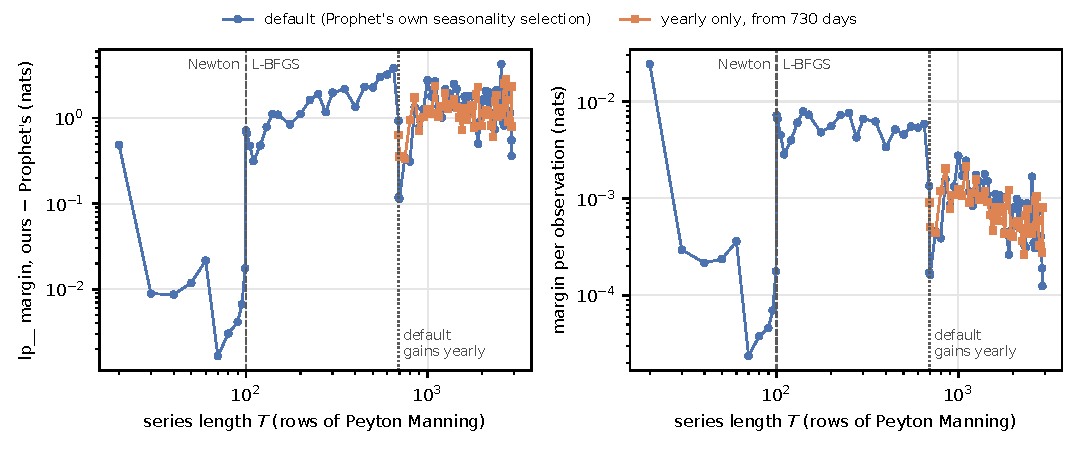
\includegraphics[width=\textwidth]{figures/margin_vs_length}
  \caption{The $\lp$ margin of the corrected optimum over Prophet's, under Prophet's
    own density, fitted on the first $T$ rows of the Peyton Manning series:
    absolute (left) and as a share of Prophet's $\lp$ (right), on logarithmic
    axes. Higher means Prophet stopped further from the optimum. Blue is Prophet's
    default seasonality selection, which adds yearly seasonality once the history
    spans 730 days, at $T = \MarginYearlyFrom$ (dotted); orange forces yearly
    seasonality alone and starts there. Left of the dashed line Prophet, and this
    implementation, run Newton's method; right of it, L-BFGS. Below $T = 33$ Prophet
    places fewer than 25 changepoints.}
  \label{fig:margin}
\end{figure}

\Cref{fig:margin} measures the margin on a finer grid: \MarginCells{} fits, at
\MarginLengths{} lengths from $T = 20$ to $2905$ in the default configuration and at
those from $T = \MarginYearlyFrom$ with yearly seasonality alone. The margin is
positive in every one of them. Its absolute size has no trend in $T$: wherever
Prophet runs L-BFGS it moves between \MarginLbfgsMin{} and \MarginLbfgsMax{} nats from
one length to the next, with a median of \MarginLbfgsMedian, while $\lp$ itself grows
roughly in proportion to $T$, so the fall of the relative margin is the growth of
its denominator. Two steps do coincide with a change in the problem or in the
solver. Where the default model gains yearly seasonality the margin falls from
\MarginBeforeYearly{} to \MarginAfterYearly{} nats. And between $T = 99$ and
$T = 100$ the data gain one observation, Prophet's solver changes from Newton to
L-BFGS, and the margin rises from \MarginAtNinetyNine{} to \MarginAtHundred{} nats.
Across the Newton range the median margin is \MarginNewtonMedian{} nats, against
\MarginLbfgsMedian{} across the L-BFGS one, so the size of the gap at short lengths is
largely a statement about which method Prophet ran.

We state the direction, which holds in every configuration measured, and claim no
mechanism for the size. It also holds across the census of \cref{sec:consequences}:
fitted on each series' full length, the corrected optimum scores higher on
\KktLpWins{} of the \KktSeries{} series, by a median of \KktLpMedian{} nats and never
by less than \KktLpMin.

Nor is the margin a matter of Prophet's stopping tolerances. Stan's L-BFGS has five
tests besides its budget of iterations, and with every one set to machine precision or
below it runs on until an iteration makes no progress or its line search fails. On the
full series that takes it from iteration \TolDefaultIterLong{} to
\TolFiveIterLong{}, and it still ends \TolFiveShortLong{} nats short of the optimum
(\TolDefaultShortLong{} at the defaults); at $T = 300$ and $1000$ it ends
\TolFiveShortShort{} and \TolFiveShortMid{} nats short, against \TolDefaultShortShort{}
and \TolDefaultShortMid. With yearly seasonality alone at $T = 2905$ it runs
\TolFiveIterYearly{} iterations instead of \TolDefaultIterYearly{} and closes the gap
from \TolDefaultShortYearly{} to \TolFiveShortYearly{} nats, and no further. These runs
call Stan directly, because where the line search fails Prophet cannot report the
result: it treats the failure as an abnormal exit and retries with Newton, passing the
tolerances on, and cmdstanpy rejects them for Newton, so the fit raises an error.

\subsection{First-order optimality}
\label{sec:evidence:kkt}

A margin in $\lp$ compares two points; a first-order certificate grades each on
its own. Write \eqref{eq:objective} as a smooth part $s$ plus
$\tau^{-1}\sum_j\lvert\delta_j\rvert$ and hold $\sigma$ at the point's own value. The
point is a minimiser if and only if $0$ lies in the subdifferential there:
$\partial s/\partial x = 0$ for $x$ among $k$, $m$ and $\beta$;
$\partial s/\partial\delta_j + \operatorname{sign}(\delta_j)/\tau = 0$ wherever
$\delta_j \ne 0$; and $\lvert\partial s/\partial\delta_j\rvert \le 1/\tau$ wherever
$\delta_j = 0$. The norm of the subdifferential's minimum-norm element measures how far
a point is from meeting them. The ``if'' is the convexity of \cref{sec:model}, which
holds in Prophet's default configuration once $\sigma$ is fixed. Fixing it costs the
argument nothing in the direction that matters: a point optimal for the full problem
is stationary in the other coordinates at its own $\sigma$, so a residual bounded
away from zero proves it is not optimal, with $\sigma$ free or not.

The gradient is Stan's, of Prophet's compiled density, through
\code{CmdStanModel.log_prob}, so neither implementation grades itself; at the
reformulation's solution it agrees with this implementation's hand-derived gradient
to $10^{-7}$. Prophet's point is read at full precision. CmdStan writes the optimum
with eight significant digits unless asked otherwise, and on \KktRoundingSeries{}
census series drawn at random that rounding alone moves Prophet's residual by up to
\KktRoundingMax, against a residual of at least \KktRoundingResidualMin{} on every one of
them.

Each of the \KktSeries{} series of the census of \cref{sec:consequences} is fitted on
its full length in Prophet's default configuration. Prophet's residual has a median
of \KktProphetStrict{}, against \KktOursMedian{} for the reformulation. The prediction
was a residual of order $1/\tau = 20$ wherever Prophet leaves a rate small but not
zero, and that is where it lies: on \KktStrictAtRate\% of series the largest violation
is a changepoint rate, of median magnitude $\KktKinkRate$, which has to balance the
prior's full slope $1/\tau$ and does not.

The obvious objection is that such a rate is zero in all but name. The relaxed
residual grants that to every rate at once, holding each $\delta_j$ only to the
condition for $\delta_j = 0$. Since $\operatorname{sign}(\delta_j)/\tau$ is an endpoint
of $[-1/\tau, 1/\tau]$, the relaxed residual is never larger than the strict one,
needs no threshold for what counts as zero, and is still a lower bound on the distance
from $0$ to the subdifferential at the point. Prophet's has a median of
\KktProphetRelaxed{} and is at least \KktProphetRelaxedMin{} on every series, so no
reading of its rates satisfies the conditions. It exceeds the reformulation's strict
residual on \KktWorse{} of the \KktSeries{} series, by a factor of \KktRatio{} at the
median and never less than \KktRatioMin. What survives the relaxation is not about the kink. On \KktRelaxedAtRate\% of
series it is a rate whose smooth gradient exceeds $1/\tau$ in magnitude, which
neither sign nor zero satisfies at that point; on \KktRelaxedAtTrend\% it is the
trend's slope or offset, which have no kink at all. On the full Peyton Manning series
Prophet's strict residual is \KktPeytonProphetStrict{} and its relaxed one
\KktPeytonProphetRelaxed{}, against \KktPeytonOurs{} for the reformulation.

The reformulation's residual is not zero either. At a median of \KktOursMedian{} it is
about one percent of $1/\tau$, and the largest across the census is \KktOursWorst{}:
the stopping tolerance of its L-BFGS-B, not exact optimality. What the certificate
establishes is the comparison, series by series, and that Prophet's points fail the
conditions under any reading of their rates.

\subsection{Scatter under convexity}
\label{sec:evidence:multistart}

With linear growth and additive seasonality the prediction is linear in
$(k, m, \delta, \beta)$ by \eqref{eq:trend}, so with $\sigma$ fixed
\eqref{eq:objective} is a quadratic in those parameters plus the convex
$\tau^{-1}\lVert\delta\rVert_1$. On the Peyton Manning series at the three lengths of
\cref{sec:evidence:lp} the design --- trend, changepoint ramps and seasonal columns ---
has full column rank, so the quadratic is strictly convex and the minimiser is
unique: a method that converges reaches it from any start, and Prophet's fits from
different starts can scatter only if Prophet's optimizer does not converge. That
argument needs no reference implementation.

We fit Prophet's own L-BFGS from \MultiStarts{} random starts at each length, with
$\sigma$ held at Prophet's own estimate. The starts are seeded: $k$ and $m$ from
$N(0, 1)$, every $\delta_j$ from Prophet's own $\mathrm{Laplace}(0, \tau)$ prior, every
$\beta_j$ from $N(0, 1)$. The fits scatter, by \MultiFixedSpreadShort,
\MultiFixedSpreadMid{} and \MultiFixedSpreadLong{} nats in $\lp$ at the three lengths,
and their rates differ from the optimum's by a median of \MultiFixedDistanceShort,
\MultiFixedDistanceMid{} and \MultiFixedDistanceLong. None of the \MultiTotal{} fits
comes within $10^{-3}$ nats of the optimum: they fall short by \MultiFixedMinShort{} to
\MultiFixedMaxShort{} nats at $T = 300$, \MultiFixedMinMid{} to \MultiFixedMaxMid{} at
$T = 1000$ and \MultiFixedMinLong{} to \MultiFixedMaxLong{} at $T = 2905$, and Prophet's
own default start is no exception, at \MultiFixedDefaultShort, \MultiFixedDefaultMid{}
and \MultiFixedDefaultLong{} nats. The optimum used to measure the distance is this
implementation's, certified with a relaxed residual of at most
$\MultiReferenceResidual$; from \MultiOurs{} of the same starts it reaches it every time,
to within $\MultiOursWorst$ nats.

With $\sigma$ free the objective is not jointly convex, and scatter there proves nothing
by itself; it is reported beside the convex case so the two are not confused. The
picture is the same. Prophet's fits fall short by \MultiFreeMinShort{} to
\MultiFreeMaxShort{} nats at $T = 300$ and \MultiFreeMinLong{} to \MultiFreeMaxLong{} at
$T = 2905$, and this implementation again reaches one point from every start. In
\MultiFallbacks{} of the free-$\sigma$ fits Stan's L-BFGS exited abnormally and Prophet's
fall-back to Newton finished it.

\subsection{Smoothing the prior inside Stan}
\label{sec:evidence:surrogate}

The most direct attribution holds everything fixed but the smoothness. We replace
$\lvert\delta_j\rvert$ in Prophet's Stan program by
$\sqrt{\delta_j^2 + \varepsilon^2} - \varepsilon$, which is zero at zero, never exceeds
$\lvert\delta_j\rvert$, and tends to it as $\varepsilon \to 0$, and fit it with Stan's
own L-BFGS: the same data, the same initialisation, the same tolerances and a fixed
seed, compiled with the CmdStan Prophet ships, whose unmodified program reproduces
Prophet's executable exactly (\cref{sec:reproducibility}). There are \SmoothValues{}
values of $\varepsilon$, from $\SmoothEpsMin$ to $1$, at the three lengths of
\cref{sec:evidence:lp}.

Measuring Stan's result against the $\ell_1$ optimum alone would mix two things: how
far Stan stops from the problem it was given, and how far that problem has moved. So
each smoothed problem is also solved independently, by a damped Newton method with the
smoothing term's Hessian exact, started both from Stan's point and from the $\ell_1$
optimum; its Newton decrement is at most $\SmoothDecrementMax$ nats in every case. Two
curves follow (\cref{fig:smoothing}). The \emph{convergence gap} is how far Stan's
L-BFGS stops short of the smoothed problem's own optimum; the \emph{smoothing bias} is
how far that optimum sits from the $\ell_1$ one. Each is scored under both densities, the
smoothed one and Prophet's.

\begin{figure}[t]
  \centering
  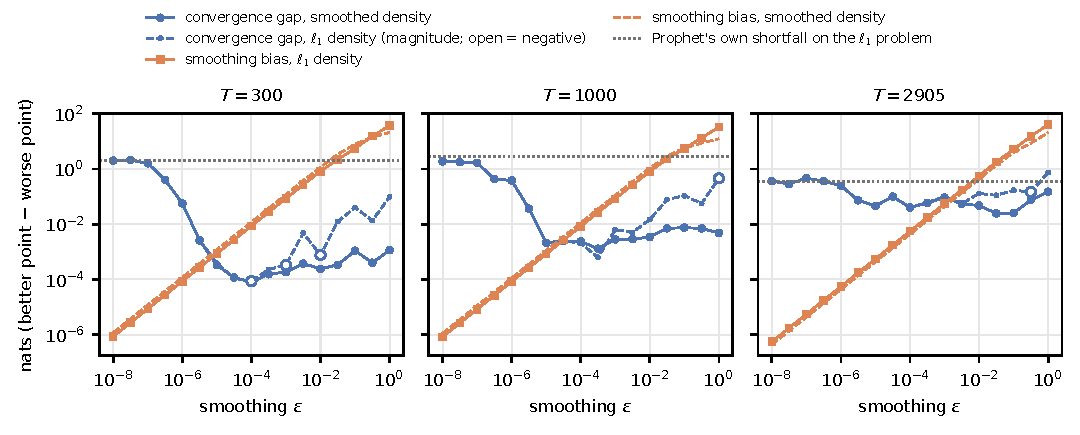
\includegraphics[width=\textwidth]{figures/smoothing}
  \caption{Prophet's Stan program with $\lvert\delta_j\rvert$ replaced by
    $\sqrt{\delta_j^2+\varepsilon^2}-\varepsilon$, fitted by Stan's own L-BFGS. Blue: the
    convergence gap, how far Stan stops short of the smoothed problem's own optimum.
    Orange: the smoothing bias, how far that optimum sits from Prophet's $\ell_1$ optimum.
    Solid lines are scored by the density each point was optimal for, dashed by the
    other; scored by Prophet's density the convergence gap is slightly negative in a few
    cells, drawn open at their magnitude. Dotted: Prophet's own shortfall on its actual
    problem. Peyton Manning, default configuration.}
  \label{fig:smoothing}
\end{figure}

At $\varepsilon = \SmoothEpsMin$ the smoothed program is Prophet's for every practical
purpose, and Stan stops short of its optimum by amounts comparable to Prophet's
shortfall on the $\ell_1$ problem: \SmoothGapAtMinShort, \SmoothGapAtMinMid{} and
\SmoothGapAtMinLong{} nats at the three lengths, against \LpMarginShort, \LpMarginMid{}
and \LpMarginLong. As $\varepsilon$
grows the convergence gap falls, by a factor of up to \SmoothDropShort, \SmoothDropMid{}
and \SmoothDropLong{} at the three lengths, while the smoothing bias rises, in proportion
to $\varepsilon$ up to $\varepsilon = 10^{-2}$, and the two cross near $\varepsilon = \SmoothCrossingShort$,
$\SmoothCrossingMid$ and $\SmoothCrossingLong$. At the best $\varepsilon$ on the grid
($\SmoothBestEpsShort$, $\SmoothBestEpsMid$ and $\SmoothBestEpsLong$), Stan's own L-BFGS on
the smoothed program lands within $\SmoothBestShort$, $\SmoothBestMid$ and
$\SmoothBestLong$ nats of Prophet's $\ell_1$ optimum --- \SmoothFactorShort, \SmoothFactorMid{}
and \SmoothFactorLong{} times closer than Prophet gets on its actual problem. Nothing but the
smoothness of the objective changed.

The gap does not vanish as $\varepsilon$ grows. Wherever $\varepsilon \ge 10^{-4}$ it
stays between $\SmoothPlateauMinShort$ and $\SmoothPlateauMaxShort$ nats at
$T = 300$, and between $\SmoothPlateauMinLong$ and $\SmoothPlateauMaxLong$ at $T = 2905$,
where Stan ends on its relative-gradient test, as it does in \SmoothStoppedGradient{} of
the \SmoothRuns{} runs. What remains there is not the kink, which the smoothed problem does
not have, but the point at which Stan's stopping rule declares a smooth problem
solved.

\paragraph{Outside Stan.}
The dependence on the kink is not peculiar to Stan's code. We ran SciPy's L-BFGS-B
\citep{byrd1995limited} with no bounds on the natural parameterisation, from Prophet's
initialisation and with its tolerances set to zero, at \StrengthLambdas{} values of
$\lambda = 1/\tau$ from $10^{-6}$ to $100$ at the three lengths. Here $\sigma$ is held at
Prophet's estimate, so that each problem is a quadratic plus
$\lambda\lVert\delta\rVert_1$ with a unique minimiser, which an active-set method
computes exactly; Stan's gradient certifies each with a relaxed residual of at most
$\StrengthReferenceResidual$. Wherever that minimiser has no rate at zero, L-BFGS
reaches it to within $\StrengthSmoothMax$ nats. As $\lambda$ grows and more of the
minimiser's rates sit on the kink, it stops further short: by \StrengthDefaultShort,
\StrengthDefaultMid{} and \StrengthDefaultLong{} nats at the default $\lambda = 20$,
where \StrengthDefaultZerosShort, \StrengthDefaultZerosMid{} and
\StrengthDefaultZerosLong{} of the 25 rates are zero. Across the \StrengthCells{} cells
the rank correlation between the shortfall and the number of zero rates is
\StrengthRankCorrelation.

\subsection{The solution path in $\tau$}
\label{sec:evidence:path}

With $\sigma$ fixed the problem is convex, and its minimiser moves continuously as $\tau$
changes --- piecewise linearly in $\lambda = 1/\tau$, as for the lasso
\citep{efron2004least}. With $\sigma$ free nothing guarantees it, but that is the setting
Prophet's users fit. We sweep $\lambda$ over \TauGlobalPoints{} values from \TauLamMin{}
to \TauLamMax{} on the Peyton Manning series in both settings. Prophet is refitted from
its own initialisation at every value, as a user changing \code{changepoint_prior_scale}
does; the exact path is computed by this implementation's Newton method on the
reformulation, warm-started from each neighbouring value and certified at every point,
with a relaxed residual of at most $\TauExactResidualMax$. Prophet's points sit a median
of \TauGapMedianFixed{} nats below the exact path with $\sigma$ fixed and
\TauGapMedianFree{} with it free, and up to \TauGapMax, with a median residual of
\TauProphetResidualMedian.

\begin{figure}[t]
  \centering
  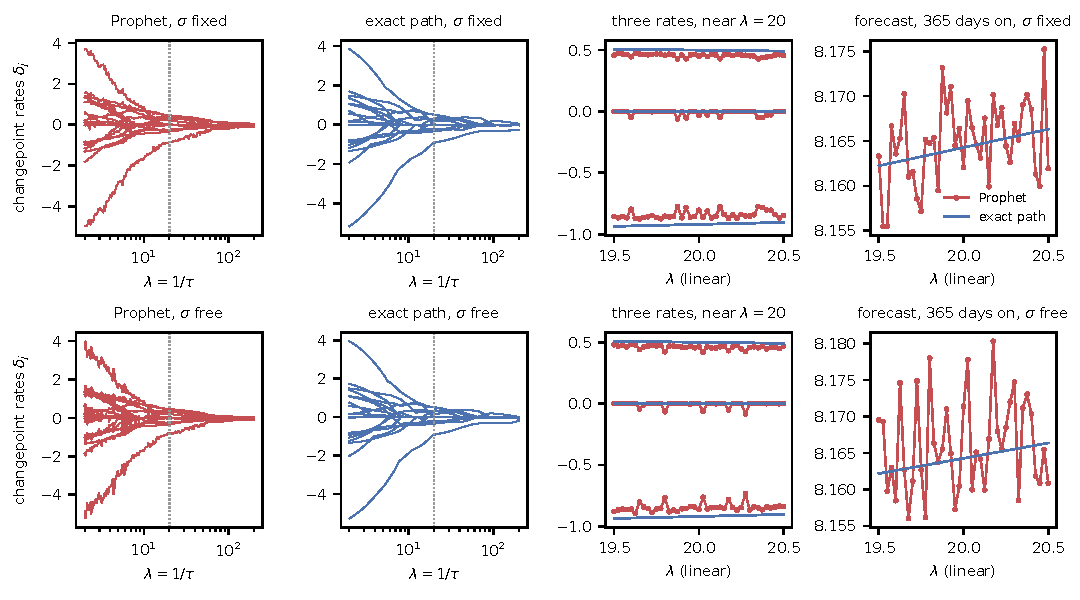
\includegraphics[width=\textwidth]{figures/tau_path}
  \caption{The solution path in $\lambda = 1/\tau$ on the Peyton Manning series. Left two
    columns: the 25 changepoint rates over the whole grid, Prophet's (Stan's L-BFGS from
    Prophet's initialisation at each $\lambda$) and the exact path. Right two columns:
    near the default $\lambda = 20$, on a grid \TauZoomStep{} apart, the three rates
    Prophet moves most and the forecast 365 days past the end of the series, both paths.
    Top row: $\sigma$ fixed, where the problem is convex; bottom row: $\sigma$ free.}
  \label{fig:tau}
\end{figure}

\Cref{fig:tau} shows a difference in kind. Near the default, on a grid \TauZoomStep{}
apart in $\lambda$, the exact path's rates move by a constant \TauExactZoomStep{} per
step, as a piecewise-linear path must, and Prophet's by as much as \TauProphetZoomMax{},
irregularly. Halving the interval of each path's largest step \TauLevels{} times, down to a
width of \TauFinalWidth{} in $\lambda$, separates steep motion from a jump: the exact
path's step halves every time, to $\TauExactFinal$, while Prophet's stays at
\TauProphetFinalFixed{} with $\sigma$ fixed and \TauProphetFinalFree{} with it free.
Prophet's path does not move steeply; it jumps, and the forecast jumps with it. This
implementation's default fit, from a cold start, stays within \TauDefaultDeviation{} of
the exact path.

\subsection{A negative control: removing the trend}
\label{sec:evidence:flat}

Under flat growth the likelihood never sees $k$ or $\delta$, so nothing pulls
against the prior and every changepoint rate goes to zero. Both implementations
then reach the same point: at each of the \FlatLengths{} lengths of
\cref{sec:evidence:lp} their $\lp$ agree to within $\FlatLpGap$ nats and their
parameters to within $\FlatParamGap$, and every one of the 25 rates is exactly zero
--- for Prophet as much as for this implementation.

This establishes that the two implementations fit the same model, so the margin
under linear growth is optimizer behaviour and not a difference of specification.
It does \emph{not} isolate the kink. Flat growth removes the ill-conditioned
$k$--$\delta$ directions and, at the same time, leaves the objective in $\delta$ as
$\tau^{-1}\sum_j\lvert\delta_j\rvert$ alone, a function every method minimises
exactly. The tie is consistent with either mechanism and the smoothing control of
\cref{sec:evidence:surrogate} is what separates them.

\subsection{One second-order method, two parameterisations}
\label{sec:evidence:newton}

To see what the kink costs a second-order method with everything else held fixed,
we run one damped Newton method on two parameterisations of the same objective. It
is this implementation's: a Hessian from central differences of the analytic
gradient, Levenberg damping, and Stan's stopping tests. On the natural
parameterisation the prior enters through its subgradient, with
$\operatorname{sign}(0) = 0$ as in Stan; on the reformulation of
\cref{sec:reformulation} it is linear. Both start from Prophet's own
initialisation, every rate at zero, on the Peyton Manning series at
\NewtonLengths{} lengths from $T = \NewtonLengthMin$ to $\NewtonLengthMax$. Only the
representation of $\delta$ differs.

On the reformulation the method reaches the optimum at every length, in
\NewtonSplitIterMin{} to \NewtonSplitIterMax{} iterations, with between
\NewtonSplitZerosMin{} and \NewtonSplitZerosMax{} of the 25 rates exactly zero. On
the natural parameterisation the same code oscillates: the rates change sign
between \NewtonFlipsMin{} and \NewtonFlipsMax{} times in a run, the progress of the
last hundred iterations falls to a median of $\NewtonProgressMin$ to
$\NewtonProgressMax$ nats a step, and Stan's stopping tests then declare
convergence, after \NewtonIterMin{} to \NewtonIterMax{} iterations, between
\NewtonShortMin{} and \NewtonShortMax{} nats short of the optimum and with no rate
exactly zero. It does not exhaust Prophet's budget of 10\,000 iterations; it stops
early and reports success.

Stan's own Newton is a different method, and it comes closer. Its Hessian is a
four-point finite difference of the gradient with a step of $10^{-3}$, wide enough
to straddle the kink wherever $\lvert\delta_j\rvert < 2\times10^{-3}$, and it damps by
reflecting negative eigenvalues rather than by adding to the diagonal. Run by
Prophet on the same series, it stops between \NewtonStanMin{} and \NewtonStanMax{}
nats short of the optimum: closer than the natural-parameterisation Newton at every
length, and at no length at the optimum, with no rate exactly zero.

\section{Consequences}
\label{sec:consequences}

Four reports in Prophet's issue tracker bear on this. Each is cited for what its
thread shows, read in full, and none is presented as an upstream report of
non-differentiability: none of them mentions it.

\paragraph{Exact sparsity and the plotting threshold.}
Prophet's changepoint rates never reach zero under linear growth, so deciding
which changepoints ``matter'' needs a cutoff; Prophet's plotting code draws those
with $\lvert\bar\delta_j\rvert \ge 0.01$. In issue~\#1422 a user reads that cutoff
as selecting the trend's breakpoints, and another participant in the thread
corrects it: the threshold is ``applied only for visualization''. We cite the
thread for the confusion, which the thread itself resolved correctly, rather than
for a defect. Under the reformulation rates reach zero exactly, and the question
answers itself.

\paragraph{Sensitivity to the prior scale.}
In issue~\#1280 a change of $2.2\times10^{-10}$ in
\code{changepoint_prior_scale} --- exactly the difference between $0.01$ and
its single-precision representation --- moved forecast accuracy by 2\%. The
headline did not reproduce; a maintainer offered as ``one possibility'' that the
optimizer ``was running into issues with one of the changepoint prior scales'',
and judged the residual variation ``inline with expectation''.
\pending{\#171}{the solution path in $1/\tau$, which is continuous for a convex
$\ell_1$ problem and is the direct test of that possibility}

\paragraph{Stalls, and the origin of the short-series rule.}
Issue~\#842 reports a ten-point series on which L-BFGS stalls indefinitely. It
is the origin of Prophet's rule that runs Newton below 100 observations, which a
maintainer added as the workaround. The maintainer diagnosed the stall as
under-identification --- plausibly so, for ten points, two changepoints, an extra
regressor and multiplicative seasonality --- and the reproducer is outside the
convex configuration of \cref{sec:model}.

Ported exactly and run on current Prophet, the reproducer no longer stalls. Under
the default rule, Newton reaches the best of \StallStarts{} random starts of this
implementation to within $\StallNewtonShort$ nats. With L-BFGS forced, Stan stops
after \StallLbfgsIter{} iterations on its parameter-change test, \StallLbfgsShort{}
nats short, at a point that fails the first-order conditions even when its rates are
read as zero (relaxed residual \StallLbfgsRelaxed). Both explanations are visible in
that stop, and they do different work. Smoothing the prior alone (\cref{sec:evidence:surrogate}),
with everything else held fixed, brings the same L-BFGS to within $\StallSmoothShort$
nats at $\varepsilon = \StallSmoothEps$: the kink is what stops it. And the shortfall
points along the softest direction of the curvature at the optimum, to a cosine of
\StallLbfgsCosine, a direction \StallCondition{} times softer than the stiffest: the
under-identification the maintainer diagnosed is what the stop costs. The variants
the thread reports as curing the stall no longer change anything. On all
\StallVariants{} of them L-BFGS stops short, by \StallVariantShortMin{} to
\StallVariantShortMax{} nats after \StallVariantIterMin{} to \StallVariantIterMax{}
iterations, Newton comes within $\StallVariantNewtonMax$, and no fit takes longer than
\StallSecondsMax{} seconds. The workaround \#842 produced is what keeps short series
on the optimum today.

This implementation does not do better here by default. The model is not convex ---
\StallStarts{} random starts reach \StallOptima{} distinct local optima, \StallBestReach{}
of them the best --- and its own default rule, which follows Prophet's to Newton, stops
at a saddle point: stationary, but with curvature $\StallOursEigen$ along one
direction, \StallOursShort{} nats below the optimum that its L-BFGS reaches. From the
same starting point Stan's Newton, which reflects negative eigenvalues of the Hessian,
reaches the optimum; this implementation's adds damping to the Hessian instead, and
stops at the saddle.

\paragraph{Non-finite log-probabilities under logistic growth.}
Issue~\#1032, opened by a maintainer, records a series under logistic growth with
multiplicative seasonality on which L-BFGS stalls and Newton fails with
\texttt{B[1] is -nan}. Reproducing it in the thread it came from (\#842), the
maintainer found L-BFGS exiting on log-probabilities of NaN and the automatic
Newton retry failing in the same way. That is outside the convex setting, and a non-finite
value is a different failure from stopping short. The thread remains open and its
mechanism is not established; we cite it as an observed failure and do not count
it as evidence for the kink.

\paragraph{Forecast accuracy.}
On the frozen census of \CensusSeries{} held-out M4 series
(\CensusWeekly{} weekly, \CensusDaily{} daily), the corrected optimum forecasts
better on \RmseWinRate\% of them by RMSE, with a median relative improvement of
\RmseAdvantage\%. The optimization defect is real and its forecast cost is
usually small.

\section{Limitations}
\label{sec:limitations}

\begin{itemize}
  \item \textbf{Per observation, the gap shrinks with series length.} The
        margin itself does not fall: wherever Prophet runs L-BFGS it moves between
        \MarginLbfgsMin{} and \MarginLbfgsMax{} nats with no trend in $T$
        (\cref{fig:margin}). Spread over the series, it falls by a factor of
        \LpPerObsDecline{} between $T = 300$ and $T = 2905$, to \LpPerObsLong{} nats
        per observation.
  \item \textbf{M4 barely exercises what Prophet is built for.} M4 records a
        domain for each series and no location, so there are no holidays to
        specify, and its starting dates were withheld from participants during
        the competition \citep{m4methods}. In this census \LimDailyModalShare\%
        of the daily series share a single starting timestamp, and there are
        \LimDailyStarts{} distinct starts among them; this implementation's loader
        also reads two-digit years so that \LimWeeklyFutureStarts{} weekly series
        start in the future. Both implementations see the same dates, so the
        comparison is unaffected, but holiday and day-of-week effects have no
        held-out evidence here at all.
  \item \textbf{Both implementations badly under-cover.} The nominal 80\%
        interval contains on average a fraction \LimCoverageOurs{} of the held-out
        points for this implementation and \LimCoverageProphet{} for Prophet:
        about a third, for both. That shared failure is larger than anything
        separating the two.
  \item \textbf{Our intervals are wider.} Across the census they are wider than
        Prophet's by a median of \LimWidthMedian\%, and wider on \LimWidthWider{} of
        the \CensusSeries{} series --- a small loss, but a consistent one.
  \item \textbf{The distribution has long tails both ways, and ours is the longer.}
        The median RMSE advantage is \RmseAdvantage\%, but on the worst series for
        this implementation its RMSE is \LimWorstCensus\% above Prophet's; on its
        best it is \LimBestCensus\% below. Restricted to the \LimPoolSize{} series
        on which both forecast to within a symmetric mean absolute percentage
        error (sMAPE) of \LimPoolThreshold, the worst is \LimWorstPool\%.
  \item \textbf{Two of M4's \LimMfourFrequencies{} frequencies.} The census is
        every weekly and daily series the protocol can measure, \CensusSeries{} of
        M4's \LimMfourSeries{} \citep{makridakis2020m4}; monthly, quarterly,
        yearly and hourly are absent.
  \item \textbf{Significance is uninformative at this $n$.} Under the sign test,
        all \LimHolmSurvivors{} of the \LimHolmComparisons{} comparisons of
        \cref{app:forecast} survive Holm adjustment, at $p$ between
        $\LimHolmMin$ and $\LimHolmMax$, which establishes only that the
        direction is consistent.
\end{itemize}

\section{Related work}
\label{sec:related}

\paragraph{Prophet and Stan.}
\citet{taylor2018forecasting} introduce the changepoint prior
$\delta_j \sim \mathrm{Laplace}(0, \tau)$ as a sparse prior for selecting
changepoints automatically, and fit the model with ``Stan's L-BFGS to find a
maximum a posteriori estimate''. \citet{carpenter2017stan} describe Stan's
optimizers, L-BFGS by default, with reference to \citet{nocedal2006numerical}, and a
run that ends as soon as any of its tolerances on the log density, the gradient or
the parameters is met. Both descriptions are accurate. This paper is about what
happens where the two meet.

\paragraph{Quasi-Newton methods on nonsmooth objectives.}
The textbook treatment of L-BFGS and Newton's method assumes smoothness
\citep{nocedal2006numerical}. \citet{lewis2013nonsmooth} study BFGS on nonsmooth
functions and find it more capable than that assumption suggests, given a line
search on the weak Wolfe condition; their suggestion that L-BFGS codes offer such a
line search is the nearest thing in that literature to the change
\cref{sec:smooth} points at. \citet{andrew2007scalable} start from the observation
that L-BFGS cannot be used as it stands for an $\ell_1$-regularised loss and modify
it, as OWL-QN, by keeping each step within an orthant. An earlier version of this
implementation used OWL-QN before the reformulation of \cref{sec:reformulation}
replaced it.

\paragraph{Methods built for the $\ell_1$ term.}
Besides orthant-wise quasi-Newton methods, cyclical coordinate descent along a
regularisation path \citep{friedman2010regularization} and iterative
shrinkage-thresholding \citep{beck2009fast} handle an $\ell_1$ penalty directly.
Each of them changes the method. The reformulation of \cref{sec:reformulation}
changes the problem instead: written as a difference of non-negative parts, the
penalty becomes linear and the bounds are left to a bound-constrained quasi-Newton
method \citep[L-BFGS-B;][]{byrd1995limited}. The device is old.
\citet[Section~6]{tibshirani1996regression} gives it, attributing it to David Gay,
as one of two algorithms for the lasso; \citet{chen2001atomic} use it to state basis
pursuit as a linear program, noting that the equivalence of minimum-$\ell_1$
problems with linear programming had been known since the 1950s; and
\citet{figueiredo2007gradient} solve the resulting bound-constrained quadratic
program by gradient projection, which is the closest in spirit to what is done
here. What \cref{sec:reformulation} adds is the statement of exactness for
Prophet's full posterior, including its non-convex configurations, and for the
local minimisers and first-order points that a solver can actually deliver.

\paragraph{Smooth reparametrisations, run inside Stan.}
The split is not the only exact way to remove the kink. \citet{hoff2017lasso} writes
each coefficient as a product, $\delta = u \odot v$, with the penalty
$\lambda(\|u\|^2 + \|v\|^2)/2$ in place of $\lambda\|\delta\|_1$. The objective becomes
smooth and unconstrained, and every local minimum in $(u, v)$ gives a local minimum in
$\delta$. \citet{kolb2026smoothing} prove the converse too: the two problems are
``equivalent in the sense of identical global and local minima''.
\citet{poon2021smooth} eliminate one factor by solving for it. For least-squares
problems they show that what remains has no spurious minima and only saddle points
that are ``ridable'', and they advocate BFGS. These are statements about the problem.
Whether a given solver finds its minimisers is a separate question, and for Prophet it
can be measured. We restated both reparametrisations in Prophet's own Stan program and
ran them on Stan's L-BFGS with Prophet's settings
(\code{paper/experiments/inside_stan.py}). In \InsideRuns{} runs, neither reaches the
optimum: the closest stops $\InsideBest$ nats short. No run sets a single rate exactly
to zero. \citet{kolb2026smoothing} say as much of gradient methods on the product form,
which have no proximal step: ``the iterates can only asymptotically approach
theoretically zero values''.

Each also needs a choice Prophet does not make. Prophet starts every rate at zero.
Setting both factors to zero gives a stationary point that is not a minimum
\citep{hoff2017lasso}, so a zero rate has to start elsewhere. From Prophet's start, the
product form then ends between $\InsideHadamardStartMin$ and \InsideHadamardStartMax{}
nats short, depending on that choice. From random starts it falls further short than
Prophet's own L-BFGS from the same starts, in median, at every length and setting; on
the full Peyton Manning series with $\sigma$ fixed it stops a median of
\InsideHadamardRandomMedianLong{} nats short of the optimum. Stan can state the split only by declaring both parts non-negative, and it
optimises such parameters through their logarithms, so a zero is approached and never
reached. Both parts of a zero rate must also start above zero. Started at $\tau$, the
split ends \InsideSplitStartMin--\InsideSplitStartMax{} nats short; at the other starting
values tried, up to \InsideSplitFloorWorst. An exact reformulation is therefore not
enough on its own. The one in \cref{sec:reformulation} reaches exact zeros because it is
solved by a method that keeps the bounds itself.

\paragraph{The lasso and its solution path.}
With $\sigma$ fixed, linear growth and additive seasonality, Prophet's MAP problem
is a least-squares problem with Gaussian penalties on $k$, $m$ and $\beta$ and an
$\ell_1$ penalty on $\delta$: a lasso-type problem \citep{tibshirani1996regression}.
For the lasso itself the solution path is piecewise linear in the penalty and can
be computed exactly \citep{efron2004least}; the lasso literature therefore offers a
standard against which a sequence of Prophet fits across $\tau$ can be read
(\cref{sec:consequences}).

\paragraph{What is not new.}
None of the methods above is ours, and neither is the observation that L-BFGS is a
poor fit for an $\ell_1$ term. The contribution is the four items listed in
\cref{sec:introduction}: a diagnosis in a specific, widely deployed system, the
controls that isolate it, an exact fix stated for that system's full model, and a
reading of its long-standing user reports against the mechanism.

\section{Reproducibility}
\label{sec:reproducibility}

Every number in the text is generated from committed results by
\code{paper/experiments/quote_numbers.py}, and the test suite fails if a section types
a number that is not one of Prophet's settings or part of an experiment's design. Every
result and figure is in turn written by a script under \code{paper/experiments/} or by
the evaluation suite, and one command, \texttt{make reproduce} in \code{paper/}, reruns
all of them and rebuilds this document. It takes hours, almost all of them spent on the
two passes over the census.

This document was built from commit \texttt{\BuildCommit} of
\url{https://github.com/adlyZaroui/analytic-prophet}. Its results were produced with
Python~\EnvPython, Prophet~\EnvProphet, cmdstanpy~\EnvCmdstanpy, NumPy~\EnvNumpy,
pandas~\EnvPandas{} and SciPy~\EnvScipy, pinned in \code{paper/requirements.txt}. Each
result records the environment and the commit it was produced at, and the test suite
holds every record to the pins. The forecast comparison uses a corpus frozen before it
was measured, identified by the digest \texttt{\CensusDigest} of its membership: a
census of every M4 weekly and daily series the protocol can measure, so there was
nothing to select.

The controls that change Prophet's Stan program
(Sections~\ref{sec:evidence:multistart}, \ref{sec:evidence:surrogate}
and~\ref{sec:evidence:path}), and the reparametrisations run inside Stan in
\cref{sec:implementation,sec:related}, compile modified copies of it, each a minimal
diff kept beside the original in \code{paper/stan/}, with CmdStan~\EnvCmdStan, the
version Prophet bundles. Compiled the same way, the unmodified program reproduces Prophet's
shipped executable exactly, in the optimum, the log density and its gradient, on both
of Prophet's optimizer paths; the test suite checks this before any variant is used.


\bibliographystyle{plainnat}
\bibliography{references}

\appendix
\section{The forecast comparison}
\label{app:forecast}

\paragraph{The census.}
The corpus is every weekly and daily series of M4 \citep{makridakis2020m4} that the
protocol below can measure, frozen before anything was measured and identified by the
digest \texttt{\CensusDigest} of its membership. A series is in it when it has at least
\CensusMinLength{} observations, a starting date that loads, and at least one
rolling-origin cutoff. Of M4's \CensusWeeklyMfour{} weekly series, \CensusWeeklyShort{}
have fewer than \CensusMinLength{} observations, and every other one yields a cutoff,
which leaves \CensusWeekly. Of its \CensusDailyMfour{} daily series,
\CensusDailyShort{} have fewer than \CensusMinLength{} observations, and
\CensusDailyNoCutoff{} more span too little calendar time to yield a cutoff, which
needs \CensusDailySpan{} days, the initial window and the horizon; that leaves
\CensusDaily. No series is lost to its starting date. The rule has no sampling step, so
nothing was selected; but it leans towards long daily series.

\paragraph{The protocol.}
Each series' cutoffs are computed once, by Prophet's own \code{generate_cutoffs}, with a
horizon, initial window and period of \CensusWeeklyHorizon, \CensusWeeklyInitial{} and
\CensusWeeklyPeriod{} weeks for weekly series and \CensusDailyHorizon,
\CensusDailyInitial{} and \CensusDailyPeriod{} days for daily ones, and handed to both
implementations. At each cutoff both are fitted on the history up to it, in Prophet's
default configuration, and forecast the horizon: Prophet through its own
\code{cross_validation}, this implementation by a fit and a predict. The two share no
fitted state; each places its changepoints by Prophet's rule, which gives the same
locations. Both are scored by Prophet's own \code{performance_metrics} with a rolling
window of one, which pools every forecast point of every cutoff into a single value per
series: MAE, RMSE, MAPE, sMAPE and the coverage of the nominal 80\% interval, beside
which the mean width of that interval is recorded. Both sides' uncertainty draws are
seeded, with \CensusSeed, so a rerun reproduces every number.

\paragraph{The comparison.}
Differences are paired per series. For the errors and the interval width the
difference is relative, this implementation's value over Prophet's minus one, so that a
series' level does not weigh on it; for coverage, a proportion, it is the plain
difference. Each is summarised by its median across the series, and tested with the test
that goes with a median, the sign test: exact and two-sided, on the series where this
implementation's value is lower against those where it is higher, with ties dropped. The
\LimHolmComparisons{} comparisons are adjusted together by Holm's procedure, and
\LimHolmSurvivors{} of them survive it (\cref{sec:limitations}), which at this $n$ says
only that the direction is consistent.
The medians and the counts carry the result: RMSE is lower on \RmseWins{} of the
\CensusSeries{} series, by a median of \RmseAdvantage\%.


\end{document}
